%% ----------------------------------------------------------------------
%% START OF FILE
%% ----------------------------------------------------------------------

\chapter{设计实现}
\label{cha:mainmatter}

\section{系统整体架构}
\label{sec:system_overview}

缓存系统的实现可分为存储卷过滤器驱动程序、缓存系统和用户配置工具几部分(图/ref{fig:sys-overview})。

\begin{figure}[htb]
\centering
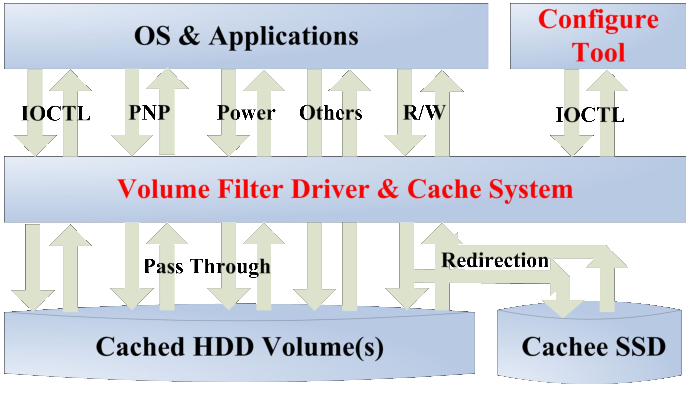
\includegraphics[width=0.6\linewidth]{./graph/sys-overview}
\caption{系统结构图}
\label{fig:sys-overview}
\end{figure}

\begin{itemize}
\item
存储卷过滤器驱动程序:过滤用户程序和操作系统对HDD卷的读写请求,供缓存算法进行SSD缓存时使用。
\item
缓存系统:完整的缓存系统实现,包括读写请求处理线程、缓存页替换算法、回写线程队列、缓存块索引数据结构等部分。
\item
用户配置工具:通过IOCTL命令与驱动程序进行交互,控制过滤器驱动程序和缓存算法的运行状态。
\end{itemize}

\begin{figure}[htb]
\centering
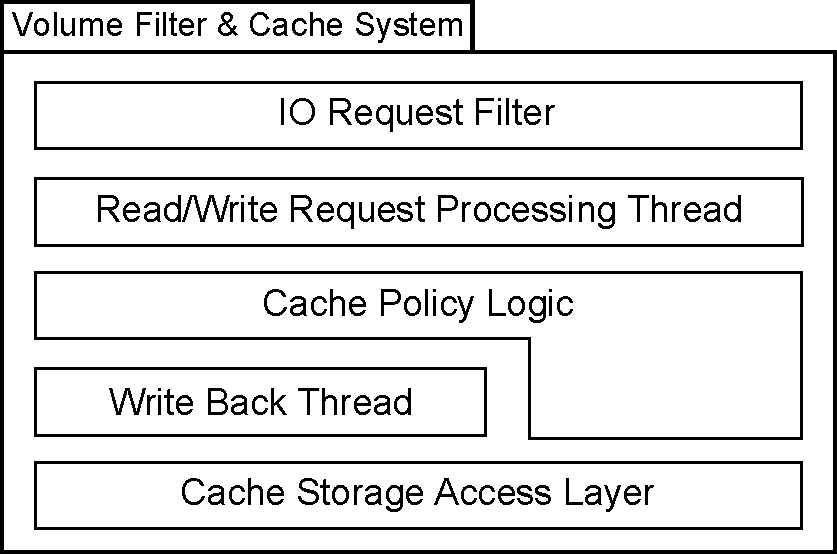
\includegraphics[width=0.6\linewidth]{./graph/sys-flt-arch}
\caption{存储卷过滤器驱动程序架构}
\label{fig:sys-flt-arch}
\end{figure}

\begin{itemize}
\item IO请求过滤器。
\item 读写请求处理线程。
\item 缓存页替换算法逻辑。
\item 回写线程。
\item 缓存介质访问层。
\end{itemize}

%% ----------------------------------------------------------------------

\section{缓存算法通用接口}
\label{sec:cache_interface}

\subsection{数据结构}
\begin{itemize}

\item 缓存块(CACHE\_BLOCK)

记录SSD缓存块和HDD存储块,最小的Cache存储单元。
\begin{lstlisting}
typedef struct _CACHE_BLOCK
{
    ULONGLONG Index;        //存储块索引,标记对应的HDD块
    ULONGLONG StorageIndex; //Cache块索引,SSD数据块指针
    BOOLEAN   Modified;     //更改标志
}CACHE_BLOCK, *PCACHE_BLOCK;
\end{lstlisting}

\item 缓存池(CACHE\_POOL)
\\Cache存储块池,用于组织存储块,记录Cache池的使用情况。
\begin{lstlisting}
typedef struct _CACHE_POOL
{
    ULONG        Size;       //Cache池总大小
    ULONG        Used;       //Cache池已使用存储块数量
    STORAGE_POOL Storage;    //存储池,管理底层存储介质访问
    ULONG32      ReadCount;  //读计数
    ULONG32      WriteCount; //写计数
    ULONG32      ReadHit;    //读命中计数
    ULONG32      WriteHit;   //写命中计数
}CACHE_POOL, *PCACHE_POOL;
\end{lstlisting}

\end{itemize}

\subsection{外部函数接口}
\begin{itemize}

\item InitCachePool
\\初始化Cache存储块池。初始化成功返回TRUE,否则返回FALSE。
\begin{lstlisting}
bool InitCachePool (
    PCACHE_POOL CachePool
);
\end{lstlisting}

\item DestroyCachePool
\\销毁Cache存储块池,释放存储空间。
\begin{lstlisting}
void DestroyCachePool (PCACHE_POOL CachePool);
\end{lstlisting}

\item QueryAndCopyFromCachePool
\\查询Cache池中的数据是否命中以Offset开始,以长度为Length的HDD数据。如果完全命中,拷贝数据到Buffer,返回TRUE;如果不命中,返回FALSE。
\begin{lstlisting}
bool QueryAndCopyFromCachePool (
    PCACHE_POOL CachePool,
    PUCHAR Buf,
    LONGLONG Offset,
    ULONG Length
);
\end{lstlisting}

\item QueryAndWriteToCachePool
\\查询Cache池中的数据是否命中以Offset开始,以长度为Length的HDD数据。如果存在命中部分,使用Buf更新Cache池中的数据,返回TRUE;如果不命中,返回FALSE。
\begin{lstlisting}
bool QueryAndWriteToCachePool (
    PCACHE_POOL CachePool,
    PUCHAR Buf,
    LONGLONG Offset,
    ULONG Length
);
\end{lstlisting}

\item ReadUpdataCachePool
\\使用Cache替换算法,利用Buffer中的数据进行Cache池的更新。Buffer中的数据是偏移为Offset,长度为Length的HDD数据。
\begin{lstlisting}
void ReadUpdataCachePool (
    PCACHE_POOL CachePool,
    PUCHAR Buf,
    LONGLONG Offset,
    ULONG Length
);
\end{lstlisting}

\item WriteUpdataCachePool
\\使用Cache替换算法,利用Buffer中的数据进行Cache池的更新。Buffer中的数据是偏移为Offset,长度为Length的最新HDD数据。为保证数据的一致性,需要替换Cache中与最新数据(偏移为Offset,长度为Length)有重叠部分的数据。
\begin{lstlisting}
void WriteUpdataCachePool (
    PCACHE_POOL CachePool,
    PUCHAR Buf,
    LONGLONG Offset,
    ULONG Length
);
\end{lstlisting}

\item IsEmpty
\\判断Cache存储块池是否为空,如果为空返回TURE;否则返回FALSE。
\begin{lstlisting}
bool IsEmpty (PCACHE_POOL CachePool);
\end{lstlisting}

\item IsFull
\\判断Cache存储块池是否已满,如果已满返回TURE;否则返回FALSE。
\begin{lstlisting}
bool IsFull (PCACHE_POOL CachePool);
\end{lstlisting}

\end{itemize}

\subsection{内部函数接口}
\begin{itemize}

\item \_QueryPoolByIndex
\\查询Cache存储块池中是否存在索引为Index的Cache块。如果存在,存放该Cache块的指针到ppBlock,返回TRUE;否则返回FALSE。
\begin{lstlisting}
bool _QueryPoolByIndex (
    PCACHE_POOL CachePool,
    LONGLONG Index,
    PCACHE_BLOCK *ppBlock
);
\end{lstlisting}

\item \_\_GetFreeBlock
\\从Cache存储块池中获取一个未使用的Cache块,如果成功获取返回空闲块指针;否则返回NULL。
\begin{lstlisting}
PCACHE_BLOCK __GetFreeBlock (PCACHE_POOL CachePool);
\end{lstlisting}

\item \_AddNewBlockToPool
\\当Cache块存储池存在空间时,加入索引为Index,数据为Data的Cache块。Modified标记传入的数据是读类型还是写类型。如果成功获取返回新创建的Cache块指针;否则返回NULL。
\begin{lstlisting}
PCACHE_BLOCK _AddNewBlockToPool (
    PCACHE_POOL CachePool,
    LONGLONG Index,
    PVOID Data,
    BOOLEAN Modified
);
\end{lstlisting}

\item \_FindBlockToReplace
\\当Cache块存储池为满时,利用Cache算法的页面替换策略从Cache池中选取出一个Cache块进行替换。Modified标记传入的数据是读类型还是写类型。如果成功获取返回数据被替换的Cache块指针;否则返回NULL。
\begin{lstlisting}
PCACHE_BLOCK _FindBlockToReplace (
    PCACHE_POOL CachePool,
    LONGLONG Index,
    PVOID Data,
    BOOLEAN Modified
);
\end{lstlisting}

\item \_IncreaseBlockReference
\\增加Cache块pBlock的引用计数。当某个Cache块被访问时(读/写),告知Cache算法其访问计数被增加。
\begin{lstlisting}
VOID _IncreaseBlockReference (
    PCACHE_POOL CachePool,
    PCACHE_BLOCK pBlock
);
\end{lstlisting}

\end{itemize}

%% ----------------------------------------------------------------------

\section{IO操作捕获函数逻辑}
\label{sec:capture_io_logic}

驱动程序通过重载卷过滤器驱动程序的分发函数达到捕获应用程序IO操作的目的。

\begin{enumerate}

\item 默认分发函数

默认分发函数用于实现我们不需要使用的分发函数接口。对于本驱动不关心的IRP,仍需传递给底层的驱动程序才能保证程序的正常运行。
一个驱动程序可以为每个分发函数接口实现一个独立的分发函数。同样的,也可以用一个分发函数实现多种分发函数接口。默认分发函数就是一种被用来实现多种分发函数接口的函数。该函数直接跳过IO栈上当前驱动设备对象所处的位置,将IRP发送给更底层的驱动设备对象(图\ref{fig:df-default})。

\begin{figure}[htb]
\centering
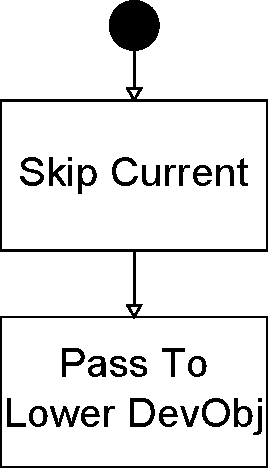
\includegraphics[width=0.2\linewidth]{./graph/df-default}
\caption{默认分发函数}
\label{fig:df-default}
\end{figure}

\item 电源事件分发函数

电源事件分发函数实现了IRP\_MJ\_POWER分发函数接口。电源事件IRP包含了操作系统对硬件设备的电源操作,或是将硬件设备的电源的状态反馈给操作系统。
Windows操作系统允许传递SystemPowerState和DevicePowerState两种类型的电源状态信息。
本论文实现的存储卷过滤器驱动程序只关注SystemPowerState的PowerSystemShutdown电源事件。如图\ref{fig:df-power}所示,当包含系统即将关机信息的IRP被捕获后,电源事件分发函数会同步所有脏缓存块到HDD,并将IRP传递给更底层的设备对象;否则,跳过当前驱动设备对象,传递IRP给更底层的驱动设备对象。

\begin{figure}[htb]
\centering
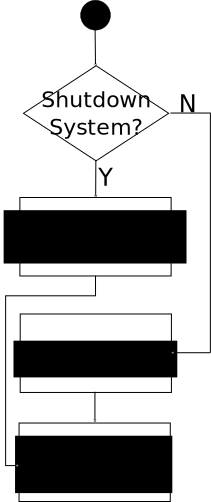
\includegraphics[width=0.3\linewidth]{./graph/df-power}
\caption{电源事件分发函数}
\label{fig:df-power}
\end{figure}

\item IOCTL分发函数

IOCTL分发函数实现了IRP\_MJ\_DEVICE\_CONTROL函数接口。IOCTL命令由Windows操作系统的IO管理器或是其他的内核驱动程序发送。大多数情况下,IOCTL类型的IRP是由用户层应用程序调用微软的Win32 API函数DeviceIoControl触发IO管理器产生的。
每当有存储卷初始化完毕将要上线时,IO管理器会给存储卷所在IO栈上的所有设备对象发送IRP\_MN\_QUERY\_REMOVE\_DEVICE的IOCTL命令。论文实现的存储卷过滤器驱动程序在过滤到此类型的IRP后,会向更底层的设备对象同步发送此IRP。确认存储卷已经上线后,检测上线的存储卷是否是目标卷。如果是目标卷,则查询目标卷的相关信息并进行相应的初始化操作,完成IRP请求;否则直接完成IRP请求(图\ref{fig:df-ioctl})。

\begin{figure}[htb]
\centering
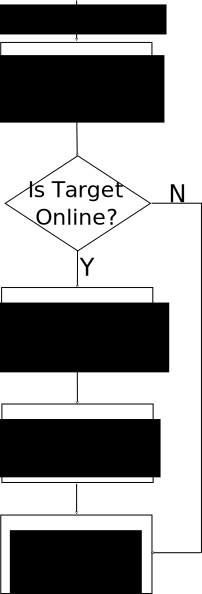
\includegraphics[width=0.3\linewidth]{./graph/df-ioctl}
\caption{IOCTL分发函数}
\label{fig:df-ioctl}
\end{figure}

\item PnP事件分发函数

PnP事件分发函数实现了IRP\_MJ\_PNP函数接口。PnP(Plug and Play)是总线在检测到硬件设备连接状态改变后,向总线驱动程序发送的一种总线信号。这种总线信号在被PnP事件管理器转换为相应类型的IRP后,会被发送给设备所在IO栈上的设备对象。
当存储卷即将被移除时,PnP事件管理器会给存储卷所在IO栈上的所有设备对象发送包含IRP\_MN\_REMOVE\_DEVICE信息的IRP。论文实现的存储卷过滤器驱动程序在过滤到此类型的IRP后,会向更底层的设备对象同步发送此IRP。确认存储卷被移除后,如果是被SSD缓存的卷,则停止工作线程、释放缓存索引占用的内存空间、从底层设备对象分离并移除当前驱动程序的设备对象,最终完成IRP请求(图\ref{fig:df-pnp})。

\begin{figure}[htb]
\centering
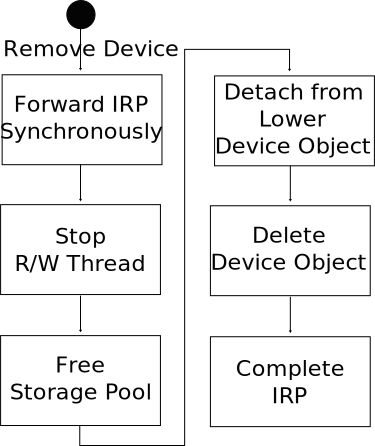
\includegraphics[width=0.4\linewidth]{./graph/df-pnp}
\caption{PnP事件分发函数}
\label{fig:df-pnp}
\end{figure}

\item 读写分发函数

存储卷的所有读和写操作都是通过IRP\_MJ\_READ和IRP\_MJ\_WRITE函数接口的实现函数完成的。论文实现的存储卷过滤器驱动程序使用一个读写分发函数统一实现了这两种函数接口。
该函数不会立即对包含读写请求的IRP进行处理(图\ref{fig:df-rw}),而是将IRP加入到驱动程序的读写请求队列中供驱动程序创建的读写线程处理,并返回IRP正在处理中的状态。

\begin{figure}[htb]
\centering
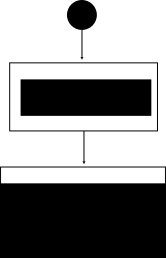
\includegraphics[width=0.2\linewidth]{./graph/df-rw}
\caption{读写分发函数}
\label{fig:df-rw}
\end{figure}

读写线程检测到读写队列不为空时,从队列头部依次处理每个读写请求(图\ref{fig:df-rw-thread})。这样做的好处是可以使并行的读写操作串行化,避免了可能的数据访问冲突,同时还可以减少锁操作对性能的消耗。

\begin{figure}[htb]
\centering
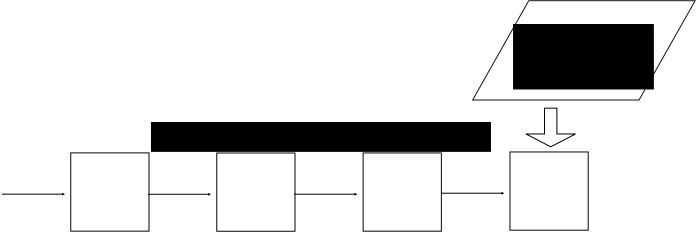
\includegraphics[width=0.5\linewidth]{./graph/df-rw-thread}
\caption{读写处理内核线程}
\label{fig:df-rw-thread}
\end{figure}

读写线程中对读和写请求的处理逻辑相似但细节不同。图\ref{fig:df-proc-read}展现了读请求的处理逻辑。

\begin{figure}[htb]
\centering
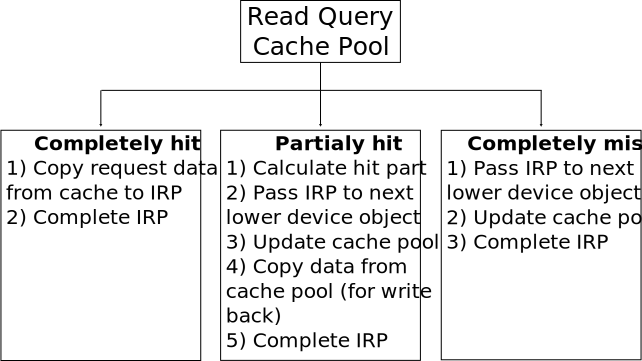
\includegraphics[width=0.75\linewidth]{./graph/df-proc-read}
\caption{读写线程读请求处理逻辑}
\label{fig:df-proc-read}
\end{figure}

图\ref{fig:df-proc-write}展现了写请求的处理逻辑。写请求和读请求的处理都存在更新SSD缓存池的操作,但实现的细节并不相同:读请求直接使用读请求获得的HDD数据更新SSD;写请求依据回写策略的不同又可分为写穿(Write Through)和写回(Write Back)两类。写穿策略会先将写请求的数据应用于HDD,再去更新SSD。写回策略直接使用写请求的数据更新SSD,回写线程负责将缓存中的脏数据同步回HDD。这两种回写策略在\ref{sec:wb_strategy}节被详细描述。

\begin{figure}[htb]
\centering
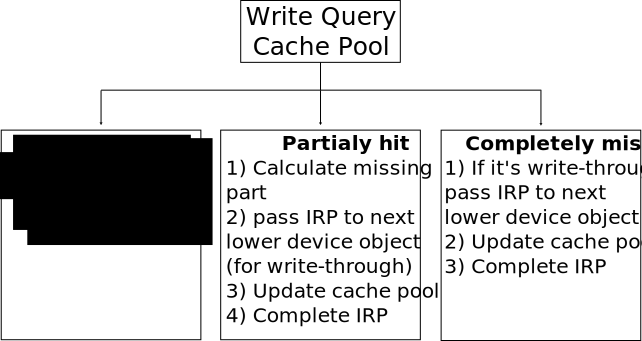
\includegraphics[width=0.75\linewidth]{./graph/df-proc-write}
\caption{读写线程写请求处理逻辑}
\label{fig:df-proc-write}
\end{figure}

\end{enumerate}

%% ----------------------------------------------------------------------

\section{用户配置工具}
\label{sec:config_utility}

系统提供了命令行的用户配置工具,在用户层和内核层的驱动程序进行交互。通过驱动设备对象提供的IOCTL命令,来完成两个方面的功能:
\begin{enumerate}
\item 配置缓存系统的运行状态。包括启动、停止和设置作为缓存的卷。
\item 获得缓存系统的统计数据。获得IO统计信息,如读写次数和命中率。
\end{enumerate}

配置工具启动后,依据用户输入的命令完成相应操作。工具提供如下几种种命令:

\begin{itemize}
\item start
\\描述:为某个指定的HDD存储卷开启SSD缓存。
\\使用:start  [disk\_number]  [volume\_number]
\\IOCTL:IOCTL\_DF\_START

\item stop
\\描述:停止某个HDD存储卷上的SSD缓存。
\\使用:stop  [disk\_number]  [volume\_number]
\\IOCTL:IOCTL\_DF\_STOP

\item stat
\\描述:获取某个存储卷的统计数据。包括读、写操作次数,缓存命中率以及使用情况。
\\使用:stat  [disk\_number]  [volume\_number]
\\IOCTL:IOCTL\_DF\_GET\_STAT

\item clear
\\描述:清除某个存储卷的统计数据。
\\使用:clear  [disk\_number]  [volume\_number]
\\IOCTL:IOCTL\_DF\_CLEAR\_STAT

\item quite
\\描述:设置驱动程序不向内核日志输出任何日志信息。
\\使用:quite
\\IOCTL:IOCTL\_DF\_QUIET

\item verbose
\\描述:开启驱动程序的向内核日志的所有日志信息输出。
\\使用:verbose
\\IOCTL:IOCTL\_DF\_VERBOSE

\item verify
\\描述:开启或关闭SSD缓存池内数据和HDD数据的一致性验证,默认是关闭的,开启对性能影响明显,只做调试使用。
\\使用:verify
\\IOCTL:IOCTL\_DF\_VERIFY

\item q
\\描述:退出用户配置工具。
\\使用:q
\end{itemize}

%% ----------------------------------------------------------------------
%%% END OF FILE
%% ----------------------------------------------------------------------